% Evaluation. Every number traces to a row of
% defense4/timing/case4_architecture/integration/core/response_only_rearm/stage_experiments/seg61_02/evaluation/CLAIM_EVIDENCE_MATRIX.md
% (row label in the trailing comment of the paragraph). Figures are mirrored by
% pipeline/sync_nomad_evidence.py from the campaign's paper-evidence directory.
\section{Evaluation}
\label{sec:evaluation}

We evaluate NOMAD against the three research objectives of Section~\ref{sec:overview}. For RO1, we measure whether the timing that the master observes equals the configured values; for RO2, we measure response sizes and protocol conformance; and for RO3, we measure the delay and the switch resources NOMAD needs. Because the objectives exist to defeat fingerprinting, we also measure what the classifier of Formby et al.~\cite{formby2016} learns from the obfuscated traffic.

\subsection{Testbed and Methodology}

\textbf{Testbed.} We run NOMAD on an Intel Tofino-1 switch with SDE~9.13.2, as three P4 programs (Appendix~\ref{app:tofino}). The DNP3 master and outstation are OpenDNP3~\cite{opendnp3} endpoints in two network namespaces of one server, connected through the same switch port, so every packet between them crosses the switch, and the outstation answers a request after a fixed 5~ms application delay. We capture every packet on the server's switch-facing interface with microsecond timestamps, once as the endpoints send it and once as the switch delivers it; the master-facing observation of Section~\ref{sec:overview} is the delivered stream.

\textbf{Configurations.} We compare four configurations on the same compiled image: \emph{No obfuscation}, \emph{Timing} (Strategies~1 and~2), \emph{Size} (Strategy~3) and \emph{Timing+Size} (all three). We vary the configured CLRT $D$ over 5, 10, 15 and 20~ms with $J$ = 2.4~ms, and the OPERATE hold $J$ over 5, 10, 15 and 20~ms with $D$ = 10~ms, i.e., eight settings, all under the one envelope of Section~\ref{sec:objectives}.

\textbf{Workload and campaign.} Each experiment block runs every configuration once, in an order that rotates between blocks, with 65 READ polls and 64 select-before-operate cycles each; we count the SELECT and the OPERATE of a cycle as two transactions. The campaign ran 154 blocks without failure, including pilot and feasibility blocks, and its 128 main blocks produced 98,816 DNP3 transactions, 16 blocks per setting. The first 8 blocks of each setting train the attackers and the last 8 test them, so no tested transaction was seen in training.

\textbf{Attacker.} We use the classifier of Formby et al.~\cite{formby2016}, a multinomial naive Bayes over 200-bin histograms of CLRT, and apply it to operations rather than device types. Its histograms have a last bin that collects every value above a threshold $H$, which we set to 1.05 times the largest training CLRT. Because the adversary reads function codes (Section~\ref{sec:overview}), it groups the CLRT values of one operation into windows of $K$ = 8, 32 and 64 transactions and classifies each window as READ, SELECT or OPERATE. Following our threat model, the attacker is trained on unobfuscated traffic captured before NOMAD is deployed and is applied afterwards. To bound what it can learn once NOMAD is in place, we also retrain the same classifier on the traffic of each configuration. In both cases, the classifier is trained on the first 8 blocks of a setting and tested on the last 8. We report balanced accuracy, for which chance among three operations is 1/3, and, for the reduction from No obfuscation to Timing+Size at $D$ = 10~ms and $J$ = 2.4~ms, a 95\% interval from 10,000 paired bootstrap resamples of the 8 test blocks. % C8, C11, C15

\subsection{RO1: Timing Replaced by Configured Values}

\begin{figure}[t]
\centering
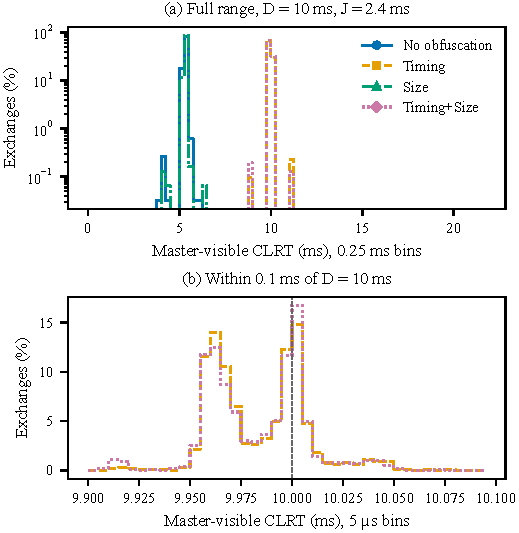
\includegraphics[width=\columnwidth]{figures/nomad_eval/fig_clrt_four_arm}
\caption{CLRT measured at the master at $D$ = 10~ms, $J$ = 2.4~ms, (a) over the full range on 0.25~ms bins and (b) within 0.1~ms of $D$ on 5~$\mu$s bins. Without timing, CLRT stays at the device's 5.3~ms; with timing, it moves to $D$.}
\label{fig:clrt}
\end{figure}

\begin{figure}[t]
\centering
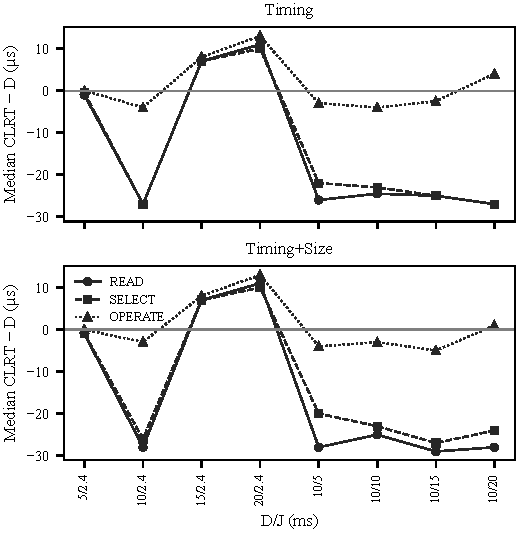
\includegraphics[width=\columnwidth]{figures/nomad_eval/fig_precision_bias}
\caption{Median signed error $\mathrm{CLRT} - D$ per setting ($D$/$J$ in ms) and operation, for Timing (top) and Timing+Size (bottom).}
\label{fig:bias}
\end{figure}


\textbf{CLRT follows the configuration.} In Fig.~\ref{fig:clrt}, we show the CLRT the master measures in every configuration at $D$ = 10~ms. Without Strategy~1, CLRT stays at the 5.3~ms the outstation needs, and response-size normalization alone leaves it there. With Strategy~1, the distribution moves to the configured 10~ms and stays within 0.1~ms of it, in two modes about 40~$\mu$s apart. Fig.~\ref{fig:precision} quantifies the error over all eight settings: the median of $|\mathrm{CLRT} - D|$ is 10--16~$\mu$s for every operation, the 99th percentile is 58--86~$\mu$s, and 0.14--0.46\% of the transactions exceed 100~$\mu$s. The few exceptions form a tail near 1~ms, with a maximum of 1.93~ms. On an earlier build, we localized this tail to a host-observed delay downstream of the switch's egress parser, and we did not re-measure that attribution on this build. % C4, C16

\begin{figure}[t]
\centering
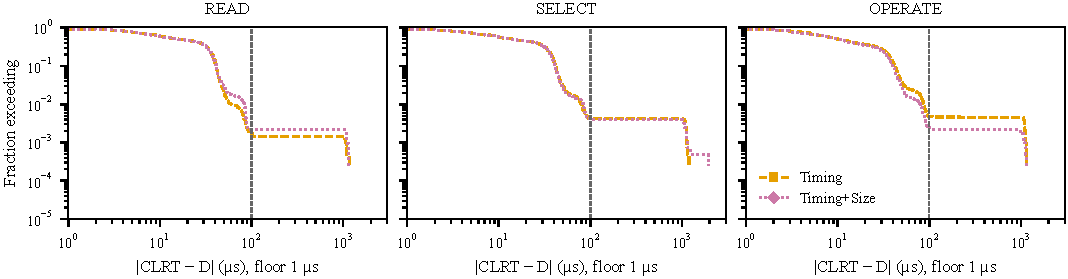
\includegraphics[width=\columnwidth]{figures/nomad_eval/fig_precision_tail}
\caption{Complementary CDF of $|\mathrm{CLRT} - D|$ for the timed configurations over all eight settings, per operation; the dashed line marks 100~$\mu$s.}
\label{fig:precision}
\end{figure}


\textbf{A small operation-dependent offset.} Fig.~\ref{fig:bias} breaks the error down by setting. At $D$ = 5, 15 and 20~ms, the three operations agree within 3~$\mu$s, at about 0, +7 and +11~$\mu$s. At $D$ = 10~ms, in all five settings of $J$, the medians of READ and SELECT sit 20--29~$\mu$s early while OPERATE stays within 5~$\mu$s of $D$; because the timed distribution has two modes (Fig.~\ref{fig:clrt}), the offset may reflect how often each operation falls in the earlier mode. We have not established the cause of this offset, which is far below the 5.3~ms CLRT of the outstation, but it is the one timing difference that remains (Section~\ref{sec:eval:attack}). % C4

\textbf{Replacement rather than shift.} A constant hold would keep the device's distribution and only move it. To show the difference, we shifted the unobfuscated CLRT at the primary setting by one constant onto the obfuscated median: the shifted OPERATE stays about 60~$\mu$s below READ and SELECT, while the measured Timing+Size distributions of the three operations lie within 25~$\mu$s of each other. The median variance of CLRT in held-out windows of 32 transactions is about three times lower with timing than without it. The native spread of our software outstation is already small, with a standard deviation of 0.06--0.11~ms, so the reduction is modest in absolute terms. % C5

\begin{figure}[t]
\centering
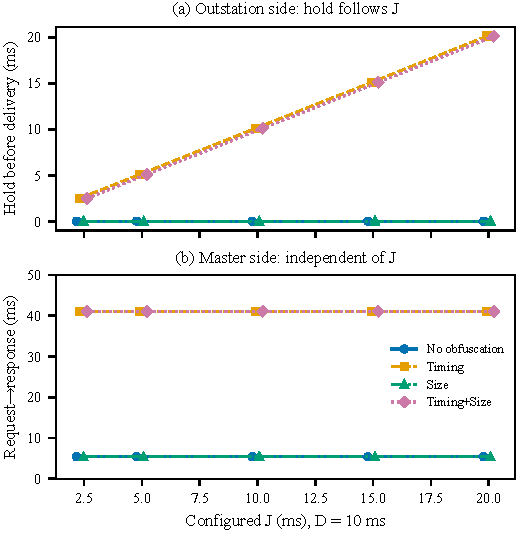
\includegraphics[width=\columnwidth]{figures/nomad_eval/fig_operate_hold}
\caption{OPERATE at $D$ = 10~ms for each $J$: (a) the hold applied before delivery to the outstation and (b) the request-to-response time at the master.}
\label{fig:operate}
\end{figure}


\textbf{The OPERATE hold stays inside the switch.} Fig.~\ref{fig:operate}(a) shows that the hold measured before delivery follows the configured $J$ in every setting. Fig.~\ref{fig:operate}(b) shows that the master nevertheless sees the same request-to-response time of 41.1~ms for every $J$, because $d_a$ covers the hold (Section~\ref{sec:strategies}). Consequently, the time a device spends on a command no longer reaches the master-facing link. % C6

\subsection{RO2: Uniform and Conformant Responses}

Table~\ref{tab:delivery} summarizes every response of the campaign. Without Strategy~3, READ responses carry 49~bytes and SELECT and OPERATE responses 37~bytes; with it, every response carries 61~bytes, and requests keep their native 20 and 35~bytes. All 98,816 responses passed the IEEE~1815 conformance checker of our harness with intact transport and application sequence numbers, and no DNP3 CRC failed. In each size-normalized configuration, 16,384 select-before-operate responses travelled as three transport frames, and the master reassembled every one of them; every READ matched the outstation's values, and every SELECT authorized its OPERATE, without any packet lost, duplicated or reordered. % C7

\begin{table}[t]
\centering
\caption{Responses per configuration over the main campaign: count, responses that passed the conformance checker, response sizes in bytes, acknowledgment commits, fallback releases, and retransmitted requests.}
\label{tab:delivery}
\footnotesize
\setlength{\tabcolsep}{3.5pt}
%% Generated by pipeline/sync_nomad_evidence.py from the campaign paper evidence; do not edit.
\begin{tabular}{lrrrrrr}
\toprule
Arm & Resp. & Conform. & Bytes & Commits & Fallb. & Retx. \\
\midrule
No obfuscation & 24,704 & 24,704 & 37/49 & 0 & 0 & 0 \\
Timing & 24,704 & 24,704 & 37/49 & 24,704 & 0 & 0 \\
Size & 24,704 & 24,704 & 61 & 0 & 0 & 0 \\
Timing+Size & 24,704 & 24,704 & 61 & 24,704 & 0 & 0 \\
\bottomrule
\end{tabular}

\end{table}

\subsection{Resistance to Fingerprinting}
\label{sec:eval:attack}

\begin{figure}[t]
\centering
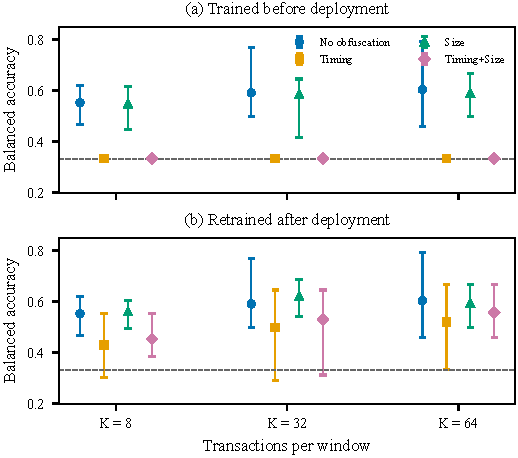
\includegraphics[width=\columnwidth]{figures/nomad_eval/fig_formby_nb}
\caption{Balanced accuracy of the classifier of Formby et al.\ per configuration and window size $K$, (a) trained before deployment and (b) retrained after deployment. Markers give the mean over the eight settings, bars the range, and the dashed line is chance.}
\label{fig:formby}
\end{figure}

\textbf{Attacker trained before deployment.} Fig.~\ref{fig:formby}(a) shows the attacker of our threat model. Without obfuscation, it identifies the operation of a window with a balanced accuracy of 0.55--0.60 on average over the eight settings, and Size alone leaves it near that level, because response sizes do not change CLRT. Under Timing and Timing+Size, it falls to 0.333 at every $K$ and in every setting, because every obfuscated window lies outside the histograms it learned from the device. At the primary setting, the reduction is 0.271 at $K$ = 8 and 32 and 0.292 at $K$ = 64, with 95\% intervals of [0.135, 0.396], [0.146, 0.396] and [0.167, 0.417]. However, a constant delay produces the same result. In a post hoc check, shifting the unobfuscated CLRT by 1~ms, or onto the median of Timing+Size, drives the same classifier to 0.33--0.36 on average over the settings. This attacker therefore fails on any timing it did not see in training, and its drop does not show that NOMAD removes operation information; the retrained attacker below is the meaningful test. % C8, C8b

\textbf{Attacker retrained after deployment.} Fig.~\ref{fig:formby}(b) shows the same classifier retrained on the traffic of each configuration. Under Timing+Size, it averages 0.454, 0.531 and 0.557 at $K$ = 8, 32 and 64, against 0.553, 0.591 and 0.604 without obfuscation, and at the primary setting the reductions are 0.130, 0.000 and $-$0.042, with intervals that include zero. Consequently, an attacker that collects labeled CLRT after NOMAD is deployed learns about as much as it learned without NOMAD in our testbed. We believe two factors explain this result. First, the unobfuscated CLRT of our software outstation barely differs between operations (Fig.~\ref{fig:clrt}), so its histograms carry little operation information to begin with. Second, the 20--29~$\mu$s offset at $D$ = 10~ms (Fig.~\ref{fig:bias}) leaves a difference that a retrained histogram can learn. Each estimate rests on 192, 48 and 24 test windows per setting at $K$ = 8, 32 and 64. % C11

\subsection{RO3: Overhead}

\begin{figure}[t]
\centering
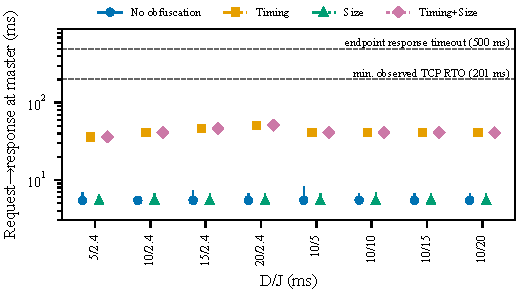
\includegraphics[width=\columnwidth]{figures/nomad_eval/fig_latency}
\caption{Request-to-response time at the master per setting ($D$/$J$ in ms), median (marker) to maximum (line), with the endpoint timers.}
\label{fig:latency}
\end{figure}

\begin{figure}[t]
\centering
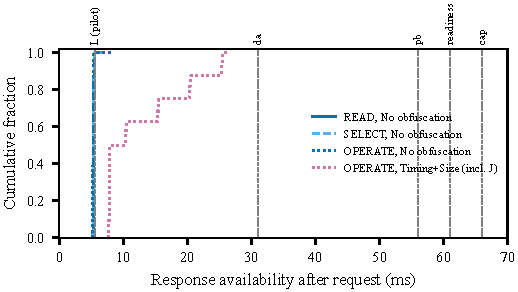
\includegraphics[width=\columnwidth]{figures/nomad_eval/fig_envelope}
\caption{Response availability after the request at the outstation side, against the envelope of Section~\ref{sec:objectives}.}
\label{fig:envelope}
\end{figure}


\textbf{Delay.} In Fig.~\ref{fig:latency}, we show the request-to-response time at the master. Without timing, a transaction completes in 5.4~ms at the median, and with timing it completes at $d_a + D$, i.e., 36.1--51.1~ms at the median, while the slowest of all 49,408 timed transactions took 52.3~ms. Every transaction completed below the 201~ms TCP retransmission timeout and the 500~ms response timeout of the master, and no request was retransmitted (Table~\ref{tab:delivery}). % C14

\textbf{Envelope coverage.} Fig.~\ref{fig:envelope} compares the time each response became available at the outstation side with the envelope. Unobfuscated responses were available within 8.0~ms and held OPERATE responses within 26.45~ms, and no response of any configuration arrived after $d_a$ = 31~ms. Consequently, every timed acknowledgment committed at its deadline, and no fallback release occurred (Table~\ref{tab:delivery}); about one blocker token for every two timed transactions outlived its packet and was retired, and delivery was unaffected. The largest availability exceeded the pilot estimate $L$ = 5.598~ms, which the guard $G$ absorbed. % C13

\textbf{Switch resources.} NOMAD fits one Tofino-1 switch, and its three programs leave most of the memory of each pipe free (Appendix~\ref{app:tofino}). % C3

\subsection{Limitations}

Our endpoints are OpenDNP3 software processes behind one switch, and the outstation answers after a fixed delay; physical relays answer with a wider timing spread, which Strategy~1 should replace the same way but which we did not measure on this build. The results are transaction-class identification by the classifier of Formby et al., which uses CLRT, not device identification. Because the adversary reads function codes, the operation of a window is already visible; the classification measures how much operation information CLRT carries, which a device fingerprint built on the same histograms would use, not information the adversary otherwise lacks. Response sizes and device-specific content such as object groups, point counts and status bits remain readable in plain text. With one outstation of nearly constant service time, RO1's independence from how fast a device serves a request follows from the design (Section~\ref{sec:strategies}), and we did not test it across devices. A device that piggybacks its acknowledgment, like the ION7550, would follow the $p_b$ path, and its master-visible timing would differ from that of a device that acknowledges separately. Our outstation sends no unsolicited responses, so we did not measure PRT, and the OPERATE hold was evaluated only on the acknowledgment and response it shapes. Holding OPERATE delays the physical execution of a command by $J$, which an operator must weigh against the timing requirements of protection functions. NOMAD leaves requests native, and their sizes alone separate READ from select-before-operate. The cause of the operation-dependent offset at $D$ = 10~ms is not established, and the guards of the envelope are margins chosen for the experiments rather than proven bounds.
